El desarrollo de este trabajo comenzó con la implementación de la estrategía Produce-and-Choose (PAC) especificado en el artículo \cite{compositeRetrival} que cuenta con una serie de algoritmos para cumplir su objetivo. La estratégia consta de dos fases que más adelante serán explicadas detalladamente. En la primer fase se producen los bundles y en la siguiente se realiza la selección de los bundles que serán parte de la solución.\\
En la producción de bundles se plantean los algoritmos del estilo \textit{Bundles One-By-One} y \textit{Hierarchical clustering}, siendo éste último modificado con respecto a la propuesta orignal del artículo. El cambio consistió principalmente en mejorar la complejidad temporal, usando nuevas estructuras de datos auxiliares, para que las pruebas puedan ser ejecutadas exitosamente con una base de datos suceptiblemente más grande. En cuanto a la fase de selección, además de las estrategias descriptas en el artículo se implementaron nuevas llamdas golosa-proporcional.\\
Adicionalmente en este trabajo se propusieron un nuevo algoritmo goloso, el cuál no comparte la estrategía de producir y luego seleccionar y dos nuevas meta huerísitcas de Búsqueda Tabú que interactúan en diferentes momentos del PAC. Una de ellas intenta encontrar mejores bundles producidos antes de comenzar con la selección final. La segunda es la encargada de mejorar la solución ya obtenida realizando intercambios de ítems dentro de la solución y con los que quedaron fuera de ella. Se aclara que esta última búsuqda toma como entrada cualquier solución sin importar el algoritmo que la generó.
\section{Modelo}
Dado el conjunto de objetos $I$ y una función de similitud $ s: I \times I \rightarrow [0;1]$, cada objeto es unívocamente identificado y contiene un conjunto de atributos. La entrada puede pensarse como un grafo completo con peso en las aristas $G=(I,E,s)$ donde el peso del vértice $(u,v)$ es $s(u,v)$. Se define también la \textit{función de distancia} $d(u,v) = 1 - s(u,v)$ que también toma valores en el intervalo $[0;1]$.

\section{Problema}
El problema consiste en devolver un conjunto de bundles $S = \left\{s_1, \ldots, s_k\right\}$ donde el bundle $S_i \in 2^{I}$ es un conjunto de objetos que satisface las reglas de \textit{complementaridad} y \textit{presupuesto}.\\
\textbf{Definición} Dado el conjunto de objetos $I=\left\{i_1,\ldots, i_n\right\}$ el bundle $S \in 2^{I}$ es válido si y sólo si satisface las reglas:
\begin{itemize}
	\item \textbf{Complementaridad:} dada la propiedad $\alpha$ de los objetos, $\forall u,v \in S_i, u.\alpha \neq v.\alpha$
	\item \textbf{Presupuesto:} dada la función de costo $f$ y el presupuesto $\beta$, entonces $\forall S_i \in S, f(S_i) \leq \beta$
\end{itemize}

La definición formal de \textit{Composite Retrieval} es:\\
Dado el conjunto de objetos $I = \left\{i_1, \ldots, i_n \right\}$, la función de similitud $s(u,v)$, el atributo complementario $\alpha$, la función de costo $f$, el presupuesto $\beta$ y el entero $k$ se desea hallar el conjunto válido de bundles $S = \left\{s_1, \ldots, s_k\right\}$ que maximiza la función:
\begin{equation} \label{des:eq-fnObj}
  \sum_{1 \leq i \leq k}{\sum_{u,v \in S_i}{\gamma s(u,v)}} + \sum_{1 \leq i \leq j \leq k}{(1-\gamma) (1-\max_{u \in S_i, v \in S_j}{s(u,v)})}
\end{equation}

En \cite{compositeRetrival} se demuestra que la complejidad de devolver $k$ bundles de items complementarios con un presupuesto es NP-Completo, por el momento no se puede encontrar una solución exacta en tiempo polinomial, por lo cual este trabajo se enfoca a encontrar soluciones suficientemente buenas para el problema. Para poder encontrar la mejor solución se implementaron dos algoritmos para poder comparar los resultados: Produce-and-Choose y algoritmo goloso.

\section{Produce-and-Choose}
El algoritmo para aproximar a la solución \texttt{Produce-and-Choose}, consiste en dos fases: En la primera fase se genera una cierta cantidad de bundles, en la fase siguiente se seleccionan los bundles que serán parte de la solución.\\
A continuación se explican los algoritmos utilizados para cada fase.
\subsection{Generación de bundles}
La generación de bundles se puede realizar a través de un proceso de agrupación de un conjunto de objetos que son parecidos. Este proceso es conocido como clustering, que consiste en agrupar objetos basándose en la información que estos describen o en sus relaciones. El objetivo es que los objetos del cluster sean similares entre sí y diferentes de los objetos de los otros grupos. Cuanto mayor es la similitud en el cluster (intra) y mayor la diferencia entre los cluster (inter) es mejor la clusterización.\\
No existe una definición formal de que es un cluster correctamente constituido porque es muy complejo realizar esta definición. Por ejemplo, para los veinte puntos de la figura \ref{res:img-howToCluster} existen tres (o más) formas de clusterizar que son válidas. Si se permite que los cluster estén acoplados, entonces la estructura de los cluster más razonable es en la que hay dos clusteres. Pero la división de los dos clusteres en tres subclusters es más intuitiva para el ojo humano. Tampoco es irracional decir que los puntos pertenecen a cuatro clusteres. Entonces la mejor definición depende del tipo de dato y del resultado esperado.

\begin{figure}[H]
  \centering
   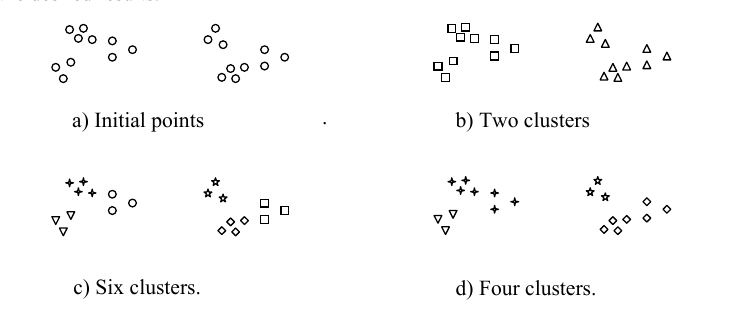
\includegraphics[width=0.8\textwidth]{img/howToCluster.png}
   \caption{}
   \label{res:img-howToCluster}
\end{figure}

En la clusterización para Composite Retrieval, la definición es que cada cluster maximice el costo que está acotado por el presupuesto, pues lo esperado es obtener cluster que utilicen el máximo del presupuesto. En cuanto al criterio utilizado para realizar la agrupación es a través de la función de similitud para que los cluster que se generan contengan los objetos, que según la función de similitud, lo más parecidos posible y de esta manera obtener bundles cohesivos.\\
Existen varios algoritmos de clustering, los cuales se pueden categorizar entre los particionales y los jerárquicos.\\
Los métodos particionales reubican iterativamente los objetos, moviéndolos de un cluster a otro. Generalmente estos métodos requieren que la cantidad de cluster a generar sea preestablecido.\\
Los métodos jerárquicos construyen los clusteres mediante la partición recursiva de los grupos de objetos. Estos métodos se pueden subdividir entre aglomerativo y divisivo. En el aglomerativo, inicialmente cada objeto representa un cluster en sí mismo y luego sucesivamente los cluster son combinados entre ellos. En el divisorio, en el inicio todos los objetos pertenecen al mismo cluster. El cluster es divido en subcluster que se siguen dividiendo en subcluster.\\
Se implementó un algoritmo de cada categoría. Del método jerárquico se desarrolló el algoritmo Hierarchical clustering, mientras que para el método de partición el algoritmo Bundles One-By-One.\\


\subsubsection{Bundles One-By-One}
El método \texttt{BOBO-k}, que está inspirado en k-means, consiste en generar $k$ cluster del conjunto de $n$ ítems. El algoritmo comienza con todos los items del conjunto $I$ como posibles pivots $P$. Se selecciona un pivote de $P$ y con los elementos de $I$ se genera un bundle válido alrededor de este. Si el bundle generado es suficientemente bueno, se agrega al conjunto de bundles candidatos y los ítems del bundle se eliminan de $I$. La generación de bundles continúa hasta que se cumpla el criterio de parada, que es la generación de $k$ bundles, o en el caso de que el valor de $k$ sea 'Ex' cuando el conjunto $P$ este vacío.

\begin{algorithm}[H]
\begin{algorithmic}[1]
\REQUIRE $I, s, \mu, k $
\ENSURE Conjunto válido de bundles
\STATE $P \leftarrow I$
\STATE $C \leftarrow \emptyset$
\WHILE {$ \left|C\right| < k\ and\ P \neq \emptyset$}
\STATE $p \leftarrow selPivote(P)$
\STATE $b \leftarrow generarBundle(D, p, s)$
\IF {$inter(b, s) \geq \mu$}
\STATE $C \leftarrow C \cup \left\{b\right\}$
\STATE $I \leftarrow I \setminus b$
\STATE $P \leftarrow P \setminus b$
\ELSE
\STATE $P \leftarrow P \setminus \left\{p\right\}$
\ENDIF
\ENDWHILE
\RETURN $C$
\end{algorithmic}
\caption{BOBO-k}\label{alg:bobo}
\end{algorithm}
Donde $I$ es el conjunto de ítems, $s$ la función de similitud, $\mu$ el umbral del valor del intra a superar por cada bundle y $k$ la cantidad de bundles a generar.

La función $selPivote$ selecciona el pivote del conjunto de pivotes. En este trabajo se siguió con la recomendación de \cite{newSimilarity} que la selección sea aleatoria. La función $generarBundle$ genera un bundle a partir del pivote. Se trata de una función que implementa un algoritmo goloso dado que que en cada iteración se agrega al bundle que se genera el ítem del conjunto $I$ que maximiza la función intra $f$ y que cumple con las restricciones de la complementaridad y el presupuesto.\\
Cuando se dice que el bundle sea suficientemente bueno significa que el valor de la intra supera un umbral establecido. O sea para el bundle $b$ se tiene que cumplir que: $\sum_{v_i, v_j \in b / i < j}{s(v_i,v_j)} \geq \mu$\\

\subsubsection{Hierarchical clustering}
La heurística Hierarchical clustering \texttt{HAC} se inicia con tantos clusters como cantidad de elementos, dado que cada cluster está conformado por un solo ítem y en cada paso se unen los dos clusters más cercanos que respetan las restricciones. Para ello se define la función de distancia para los ítems $u$ y $v$ como:\\

\begin{equation} \label{des:eq-dist-d1}
d_{1}(u,v) = 1 - s(u, v)
\end{equation}

Los cluster que se generan a partir de la función de distancia $d_{1}$ 

Con la  se generan los cluster lo más cohesivos posibles.\\
En la figura \ref{des:img-usingEfficientHAC} se observa que el algoritmo selecciona los ítems más cercanos. En las búsquedas que se realizan en \cite{compositeRetrival} se tiene el parámetro $\gamma$ que indica que tipo de resultado es el esperado.

\begin{figure}[H]
  \centering
    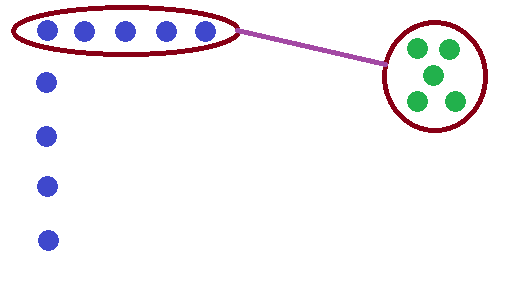
\includegraphics[width=0.3\textwidth]{img/cluster2.png}
  \caption{Selección de bundles usando $d_{1}$}
  \label{des:img-usingEfficientHAC}
\end{figure}

En caso de que el $\gamma$ sea pequeño, la clusterización esperada para la misma instancia es la que se visualiza en la imagen \ref{des:img-usingSingleHAC}, clusters no tan cohesivos pero más variados. Por lo que se define una función de distancia que considera el $\gamma$.\\

\begin{equation} \label{des:eq-dist-d2}
d2(u,v) = 1 - FO(\{u\} \cup \{v\})
\end{equation}
Donde $FO$ es la función definida en \ref{des:eq-fnObj} \\

\begin{figure}[H]
  \centering
    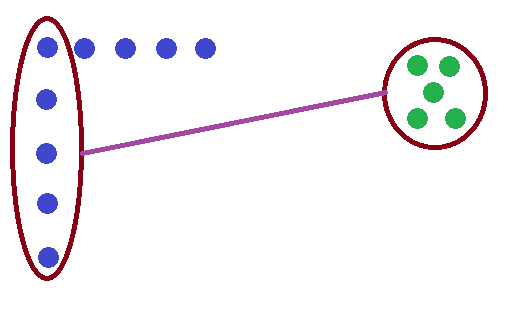
\includegraphics[width=0.3\textwidth]{img/cluster1.png}
  \caption{Selección de bundles usando $d_{2}$}
  \label{des:img-usingSingleHAC}
\end{figure}

Para la distancia $d_{1}$ \ref{des:eq-dist-d1} se implementó el algoritmo \texttt{EfficientHAC} que es tiene una complejidad $\mathcal{O}(n^{2})$, mientras que para $d_{2}$ \ref{des:eq-dist-d2} el algoritmo es \texttt{SingleHAC} que la complejidad es $\mathcal{O}(n^{2} * \ln{n})$. Según se demostró en el capítulo 17 de \cite{informationRetrival}.


\subsection{Selección de bundles}
Al finalizar la producción de bundles, se deben seleccionar los $k$ bundles para la solución. El problema de seleccionar los bundles que maximizan la función objetivo, se traduce en encontrar en el grafo G el k-subgrafo de mayor peso de nodos y vértices. Dónde el peso de los nodos representa la calidad de los bundles y el peso de las aristas es la distancia entre los nodos.\\
Formalmente el problema de encontrar el subgrafo de máximo peso de nodos y vértices con k nodos, consiste en dado el grafo $ G = (V,E) $, la funciones de peso $\psi : E \rightarrow \Re$ y $\omega : V \rightarrow \Re$, el entero $ k \leq |V| $ y el real $\gamma \in [0,1]$. La salida es el conjunto $V' \subseteq V$ tal que $|V'| = k$ que maximiza el peso de los nodos y vértices del subgrafo $G' = (V', E')$ ponderado por el parámetro $\gamma$.

\begin{equation}
\gamma \sum_{v \in V'}{\omega(v)} + (1 - \gamma) \sum_{(u,v) \in E'}{\psi(u,v)}
\end{equation}

El problema de encontrar el máximo k-subgrafo con pesos en los nodos y vértices, se puede reducir al problema ya conocido de hallar el k-subgrafo más denso\cite{SubgraphProblem}. Transformando en la instancia del problema original la función del peso de los vértices por:
 
\begin{equation}
\omega(u,v) = \dfrac{\gamma}{2( k - 1)} (\omega(u) + \omega(v)) + (1 - \gamma)\psi(u,v) 
\end{equation}

A esta nueva instancia del problema, se le aplica la heurística golosa en la que en cada iteración se remueve el nodo con menos peso en las aristas.\\

\begin{algorithm}[H]
\begin{algorithmic}[1]
\REQUIRE $k, \alpha,$ el grafo con peso en los vértices y aristas  $G=(V,E)$ donde $\forall S \in V / \omega(S) = \sum_{u,v \in S}{s(u,v)}$ y $\forall (S_i,S_j) \in E / \psi(S_i,S_j) = 1 - \max_{u \in S_i, v \in s_j}{s(u,v)}$
\ENSURE Conjunto de k bundles
\STATE $\omega(u,v) = \dfrac{\gamma}{2( k - 1)} (\omega(u) + \omega(v)) + (1 - \gamma)\psi(u,v)$
\STATE $S \leftarrow V$
\WHILE {$ \left|S\right| > k$}
\STATE $u \leftarrow \min_{u \in S}{\sum_{v \in S}{\omega(u,v)}}$
\STATE $S \leftarrow S \setminus  \left\{u\right\} $
\ENDWHILE
\RETURN $C$
\end{algorithmic}
\caption{Selección de bundles}\label{alg:chooseBundles}
\end{algorithm}

Otra heurística propuesta para la selección (también golosa) en lugar de ir descartando los bundles, la solución se genera agregando un bundle en cada iteración. Los valores del intra al ser mayores que los de inter, por lo tanto para mantener la relación del $\gamma$ inter-intra durante todo el proceso el cálculo que se realiza para seleccionar el bundle es proporcional a la iteración actual. De esta manera se asegura que en las primeras iteraciones el valor del intra no haga despreciable al inter en el momento de realizar la selección.\\
Sea $B$ el conjunto de bundles producidos y $S \subseteq B$ el conjunto de bundles seleccionados en la iteración $i$ se agrega a la solución el bundle que cumple con:

\begin{equation}
\max_{b \in (B/S)}{\dfrac{k}{|S|}} \gamma \sum_{v \in \left\{b\right\} \cup S}{\omega(v)} + \dfrac{k * (k-1)}{|S| * (|S|-1)} (1-\gamma) \sum_{v,w \in \left\{b\right\} \cup S}{\psi(v,w)}
\end{equation}

\begin{algorithm}[H]
\begin{algorithmic}[1]
\REQUIRE $B, k$
\ENSURE Conjunto de k bundles
\STATE $S \leftarrow V$
\WHILE {$ \left|S\right| < k$}
\STATE $c \leftarrow \max_{b \in (B/S)}{\dfrac{k}{|S|}} \gamma \sum_{v \in \left\{b\right\} \cup S}{\omega(v)} + \dfrac{k * (k-1)}{|S| * (|S|-1)} (1-\gamma) \sum_{v,w \in \left\{b\right\} \cup S}{\psi(v,w)}$
\STATE $S \leftarrow S \cup \left\{c\right\}$
\STATE $B \leftarrow B \setminus \left\{c\right\}$
\ENDWHILE
\RETURN $S$
\end{algorithmic}
\caption{Selección de bundles proporcional}\label{alg:algSelProp}
\end{algorithm}

\section{Algoritmo goloso}
En los algoritmos previos se centraron en construir bundles maximizando el intra y una vez generado una cantidad suficiente seleccionar un conjunto de estos para la solución. En el algoritmo goloso propuesto, se generan únicamente los bundles que pertenecen a la solución. Agregando iterativamente el item al bundle que maximiza la función objetivo.\\
El algoritmo comienza con los bundles de la solución vacíos. En cada paso selecciona, de los items que no son parte de la solución, aquel que máximiza la función objetivo agregándolo a alguno de los bundles sin violar las restricciones del problema.

\begin{algorithm}[H]
\begin{algorithmic}[1]
\REQUIRE $numOfSnowFlakes:Integer$
\ENSURE $selected:Vector<SnowFlake>$
\STATE $selected_{i}:Vector<SnowFlake> \leftarrow \emptyset_{0\leq i<numOfSnowFlakes}$
\STATE $isComplete:Bool \leftarrow False$
\STATE $elements:Set<Element> \leftarrow ElementsOfTheProblem$
\WHILE {$isComplete == False$}
  \STATE $bestScore:Double \leftarrow -\infty$
  \STATE $bestElement:Element \leftarrow \varnothing$
  \STATE $bestBundle:SnowFlake \leftarrow \varnothing$
  \FOR {$elem:Element \in elements$}
    \FOR {$bundle:SnowFlake \in selected$}
      \IF {$isValidBundle(bundle \cup \{elem\}) == True$}
        \STATE $score:Double \leftarrow FO(selected.replace(bundle, bundle \cup \{elem\}))$
        \IF {$score > bestScore$}
          \STATE $bestScore \leftarrow score$
          \STATE $bestBundle \leftarrow bundle$
          \STATE $bestElement \leftarrow elem$
        \ENDIF
      \ENDIF
    \ENDFOR
  \ENDFOR
  \STATE $selected \leftarrow selected.replace(bundle, bundle \cup \{elem\})$
  \STATE $elements.erase(elem)$
  \STATE $isComplete \leftarrow bestElement == \varnothing$
\ENDWHILE
\RETURN $selected$
\end{algorithmic}
\caption{Algoritmo heurística golosa}\label{alg:algHeuGol}
\end{algorithm}

\section{Búsquedas Tabú}
Las búsquedas locales consisten en moverse de solución en solución, aplicando cambios a la solución candidata hasta encontrar una mejor solución o satisfacer un criterio de parada. Los algoritmos consisten en comenzar con una solución e iterativamente moverse a una solución vecina, esto es posible solo si se pude definir una relación de vecindad en el espacio de búsqueda. Como una solución puede tener muchas soluciones vecinas se elige siempre la que maximice o minimice (según el problema elegido) el criterio seleccionado, esto produce que el algoritmo pueda estancarse en un mínimo (ó máximo) local y nunca pueda salir de él.\\
\textbf{Tabú search} es una metaheurística, de la familia de las búsquedas locales, que relaja la primer regla de las búsquedas locales tradicionales y permite moverse a una solución vecina que no cumple con el criterio de búsqueda. De esta manera se permite al algoritmo escapar de máximos o mínimos locales y encontrar una mejor solución (en caso que existiese). Otras de las modificaciones que se agregan es que una vez que una solución determinada es visitada, se la marca como tabú para que no vuelva a ser visitada por una determinada cantidad de iteraciones para también de esta manera evitar caer en ciclos y mínimos o máximos locales.\\
Una de las ventajas que tienen este tipo de metaheurísticas es que no son muy costosas en tiempo de ejecución siempre que la cantidad máxima de iteraciones no sea excesiva, con lo cual se puede ejecutar sin problemas y sin importar el algoritmo de generación y selección provenga la solución orginal con el fin de intentar mejorarla.\\
Se implementaron las búsquedas tabú Inter-Bundle e Intra-Bundle. La primera busca encontrar una mejor solución entre la solución actual y los bundles ya generados; la otra consiste en mejorar los bundles con los items que quedaron fuera de la solución.

\subsection{Inter-Bundle}
La búsqueda se concibió especialmente para la fase de selección del algoritmo \texttt{Produce and Choose}. En esta fase se eligen los bundles que pertenecen a la solución. De la solución obtenida se realiza la búsqueda tabú con los bundles generados en la fase del produce con el objetivo de recorrer las soluciones con bundles menos cohesivos entre si.\\
Los movimientos de la solución $S$ a la solución $S'$ consiste de los siguientes  pasos:
\begin{enumerate}
	\item Obtener el Bundle de la solución a reemplazar.
	\item Determinar el bundle centroide de la solución.
	\item Agregar a la solución el bundle más alejado al centroide.
\end{enumerate}

Sea $S$ el conjunto de bundles de la solucion y B el conjunto de todos los bundles producidos. El bundle (1) es el más acoplado al de la solución $b_r = \min_{b_1 \in S}{\sum_{b_2 \in S}{\psi(b_1,b_2)}}$. El centroide de (2) es el bundle que tiene mayor similitud entre los bundles de la solución, sin tener en cuenta al bundle a reemplazar, entonces el centroide es:
$$b_c = \min_{b_1 \in S \setminus \left\{b_r\right\}}{\sum_{b_2 \in S \setminus \left\{b_r\right\}}{\psi(b_1,b_2)}}$$
El bundle de (3) se obtiene de $b_n = \min_{b_1 \in S \setminus \left\{b_r\right\}}{\psi(b_1,b_c)}$. Por lo tanto la nueva solución es $S' = (S \setminus \left\{b_r\right\}) \cup \left\{b_n\right\}$. Mientras que el bundle $b_r$ se marca para que no sea seleccionado para las próximas soluciones generadas.
\begin{algorithm}[H]
\begin{algorithmic}[1]
\REQUIRE $aSolution: Vector<SnowFlake>, $\\
         $remainingBundles: Vector<SnowFlake>, gamma: Double$
\ENSURE $newSolution:Vector<SnowFlake>$
\STATE $iteration:Integer \leftarrow 0$
\STATE $tabuBundles: Set<SnowFlake>$
\STATE $bestSolution: Vector<SnowFlake> \leftarrow aSolution$
\STATE $bestFunction:Double \leftarrow FO(bestSolution)$
\STATE $tempSolution: Vector<SnowFlake> \leftarrow bestSolution$
\WHILE {$iteration < MAX\_ITER$}
  \STATE $updateTabuCount(tabuBundles)$
  \STATE $iterationSolution: Vector<SnowFlake> \leftarrow tempFunction$
  \STATE $worstBundle: SnowFlake \leftarrow$\\
         $getWorstBundle(iterationSolution, tabuBundles)$
  \STATE $centroidBundle: SnowFlake \leftarrow findCentroid(iterationSolution)$
  \STATE $bestBundles: Set<SnowFlake> \leftarrow findBestBundles($\\
         $centroidBundle, remainingBundles, tabuBundles)$
  \STATE $interFunction: Doubel \leftarrow calculateInter(iterationSolution)$
  \FOR {$aBundle \in bestBundles$}
    \STATE $iterationSolution.replace(worstBundle, aBundle)$
    \STATE $newInterFunction \leftarrow calculateInter(iterationSolution)$
    \IF {$newInterFunction > interFunction$}
      \STATE $betterSolution: Bool \leftarrow True$
      \STATE $saveSolution$
    \ELSE
      \IF {$not betterSolution$\\
           $and\ otherFunction\ is\ better\ than\ others\ functions$\\
           $and\ aBundle\ was\ tabu\ before$}
        \STATE $bestWorstSolution: Bool \leftarrow True$
        \STATE $saveSolution$
      \ENDIF
    \ENDIF
  \ENDFOR
  \IF {$betterSolution$}
    \STATE $replace\ tempSolution\ with\ saved\ solution$
    \STATE $newFunction: Double \leftarrow FO(tempSolution)$
    \IF {$newFunction > bestFunction$}
      \STATE $bestSolution \leftarrow tempSolution$
    \ENDIF
  \ELSE
    \IF {$bestWorstSolution$}
      \STATE $replace\ tempFunction\ with\ saved\ solution$
    \ENDIF
  \ENDIF
  \STATE $tabuBundles \leftarrow tabuBundles \cup {worstBundle}$
\ENDWHILE
\STATE $newSolution \leftarrow bestSolution$
\RETURN $newSolution$
\end{algorithmic}
\caption{Algoritmo búsqueda tabú sobre bundles}\label{alg:algBusTabuBundle}
\end{algorithm}

\subsection{Intra-Bundle}
En Intra-Bundle explora soluciones con bundles más cohesivos. De la solución actual se realiza el movimiento a una nueva solución con los pasos:
\begin{enumerate}
	\item Obtener el bundle menos cohesivos de la solución.
	\item Determinar el centroide del bundle.
	\item Hallar el ítem más alejado del centroide.
	\item Reemplazar con el ítem, que no pertenece a la solución, más cercano al centroide.
\end{enumerate}

Sea $S$ el conjunto de bundles de la solución e $I$ el conjunto de ítems, el bundle de (1) es $b = \min_{b_1 \in S}{\sum_{v,w \in b_1}{s(v,w)}}$. De $b$ se define el centroide $c$ del paso (2) con $c = \max_{v \in b}{\sum_{w \in b}{s(v,w)}}$. El item de (3) se obtiene de $i = \min_{v \in b}{s(v,c)}$. El item para reemplazar a $i$ es $j = \max_{v \in I \setminus items(S)}{s(v,c)}$. Por lo que la nueva solución se define $S' = (S \setminus \left\{b\right\}) \cup \left\{(b \setminus \left\{i\right\})\cup\left\{j\right\}\right\}$

\begin{algorithm}[H]
\begin{algorithmic}[1]
\REQUIRE $aSolution: Vector<SnowFlake>, gamma: Double$
\ENSURE $newSolution:Vector<SnowFlake>$
\STATE $iteration:Integer \leftarrow 0$
\STATE $tabuBundles: Set<SnowFlake>$
\STATE $tabuElements: Set<Element>$
\STATE $bestSolution: Vector<SnowFlake> \leftarrow aSolution$
\STATE $bestFunction:Double \leftarrow FO(bestSolution)$
\STATE $tempSolution \leftarrow bestSolution$
\WHILE {$iteration < MAX\_ITER$}
  \STATE $updateTabuCount(tabuBundles)$
  \STATE $updateTabuCount(tabuElements$
  \STATE $bundeWithWorstInter: SnowFlake \leftarrow$\\
  $findWorstIntraBundle(tempSolution, tabuBundles)$
  \STATE $centroid: Element \leftarrow findCentroid(bundeWithWorstInter)$
  \STATE $farAwayElement: Element \leftarrow$\\
  $findFarAwayElement(centroid, bundeWithWorstInter)$
  \STATE $bestElements: Set<SnowFlake> \leftarrow$\\
  $nearestElements(centroid, farAwayElement, bundeWithWorstInter, tabuElements)$
  \STATE $tempFunction: Double \leftarrow FO(tempSolution)$
  \FOR {$near:Element \in bestElements$}
    \STATE $newBunlde: SnowFlake \leftarrow bundeWithWorstInter.replace(farAwayElement, near)$
    \STATE $otherSolution: Vector<SnowFlake> \leftarrow$\\
    $tempSolution.replace(bundeWithWorstInter, newBunlde)$
    \STATE $otherFunction: Double \leftarrow FO(otherSolution)$
    \IF {$otherFunction > tempSolution$}
      \STATE $betterSolution: Bool \leftarrow True$
      \STATE $saveSolution$
    \ELSE
      \IF {$not betterSolution$\\
           $and\ otherFunction\ is\ better\ than\ others\ functions$\\
           $and\ bundeWithWorstInter\ was\ tabu\ before$}
	\STATE $bestWorstSolution: Bool \leftarrow True$
	\STATE $saveSolution$
      \ENDIF
    \ENDIF
  \ENDFOR
  \IF {$betterSolution$}
    \STATE $replace\ tempSolution\ with\ saved\ solution$
    \STATE $newFunction: Double \leftarrow FO(tempSolution)$
    \IF {$newFunction > bestFunction$}
      \STATE $bestSolution \leftarrow tempSolution$
    \ENDIF
    \STATE $tabuElements \leftarrow tabuElements \cup {farAwayElement}$
  \ELSE
    \IF {$bestWorstSolution$}
      \STATE $replace\ tempSolution\ with\ saved\ solution$
      \STATE $tabuElements \leftarrow tabuElements \cup {farAwayElement}$
    \ENDIF
  \ENDIF
\ENDWHILE
\STATE $newSolution \leftarrow bestSolution$
\RETURN $newSolution$
\end{algorithmic}
\caption{Algoritmo búsqueda tabú sobre elementos}\label{alg:algBusTabuIntra}
\end{algorithm}
